\documentclass{article}
\usepackage{graphicx}
\usepackage{verbatim}

\graphicspath{{images/}}
 
\begin{document}

\begin{figure}[h]
    \centering
    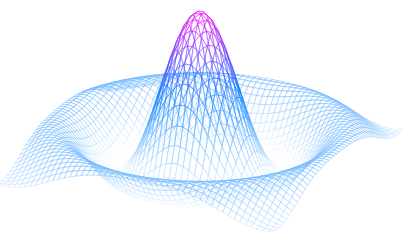
\includegraphics[width=0.75\textwidth]{mesh}
    \caption{A nice plot.}
    \label{fig:mesh1}
\end{figure}
 
As you can see in figure \ref{fig:mesh1}, the function grows near the origin. This example is on page \pageref{fig:mesh1}.

\begin{comment}
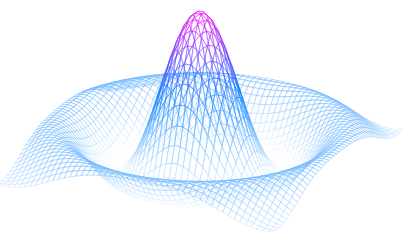
\includegraphics[width=0.75\textwidth]{mesh}: This form of \includegraphics instructs LaTeX to set the figure’s width to 75% of the text width—whose value is stored in the \textwidth command.
\caption{A nice plot.}: As its name suggests, this command sets the figure caption which can be placed above or below the figure. If you create a list of figures this caption will be used in that list.
\label{fig:mesh1}: To reference this image within your document you give it a label using the \label command. The label is used to generate a number for the image and, combined with the next command, will allow you to reference it.
\ref{fig:mesh1}: This code will be substituted by the number corresponding to the referenced figure.

\end{comment}

\end{document}

% There are several noteworthy commands in the example:

